\documentclass[10pt,a4paper]{article}
\usepackage[CJKchecksingle,CJKnumber]{xeCJK}
\usepackage{graphicx}
\usepackage{float}
\usepackage{fancyhdr}
\usepackage{amsfonts}
\usepackage{setspace}
\usepackage{booktabs}
\usepackage{listings}
\usepackage{geometry}
\geometry{left=2.5cm,right=2.5cm,top=4cm,bottom=2cm}
\lstset{numbers=left,
	numberstyle=\tiny,
	keywordstyle=\color{blue!70}, commentstyle=\color{red!50!green!50!blue!50},
	frame=shadowbox,basicstyle=\ttfamily,
	rulesepcolor=\color{red!20!green!20!blue!20}
}
\usepackage[svgnames, table]{xcolor}
\usepackage[bookmarksnumbered, pdfencoding=auto, pdfpagelayout=TwoPageRight,
breaklinks, colorlinks, linkcolor=blue, urlcolor=blue]{hyperref}
\usepackage{indentfirst}
\setlength\parindent{2em}
\usepackage{tikz}
\usepackage{amsmath}
\usetikzlibrary{matrix,calc}
\newcommand{\horrule}[1]{\rule{\linewidth}{#1}} % Create horizontal rule command with 1 argument of height
\pagestyle{fancy}
\rhead{Advanced Applications of Machine Learning}

\title{	
	\normalfont \normalsize
	\textsc{Department of Electronic Engineering} \\ [25pt]
	\horrule{0.5pt} \\[0.4cm] % Thin top horizontal rule
	\huge Computational Classification of circular RNA from other non-coding RNA using LSTM\\ % The assignment title
	\horrule{2pt} \\[0.5cm] % Thick bottom horizontal rule
}
\author{ Liwei Cai 2014011255\\
	Kaidi Cao 2014012282 } % Your name

\date{\normalsize\today} % Today's date or a custom date

\begin{document}
	
	\begin{spacing}{1.5}
		\begin{titlepage}
			\maketitle % Print the title
		\end{titlepage}
		
		\newpage
		
		\section{Introduction}
		
		To the best knowledge of us, nowadays we can easily distinguish lncRNA from other small ncRNAs, such as miRNA, siRNA and snoRNA, by using the simple property transcript size. However, it has been studied that the identification of circular RNA from other lncRNAs is not a trivial work. Though we've learned that circular RNAs have demonstrated some different sequence characteristics from other lncRNAs, such as GT-AG pair of canonical splice sites, paired ALU repeats and backspace, it is still almost impossible to detect circular RNAs using simple features. 
		
		On the other hand, sequence-based method have been shown to maintain the potential to be utilized in the identification of circular RNAs. In this project, we try to implement LSTM, which is a quite popular approach in the domain of natural language processing. 
		
		\section{Related Work}
		
		Basically we don't have enough time to evaluate all the papers published aiming at cope with this problem. [1] and [2] all use pre-extracted features from RNA sequences and implement classifier upon those features. However, they didn't demonstrate explicitly how they extract more than 100 features from scratch. What's more, we students from EE are not able to distinguish the essential difference between circular RNA and lncRNA, so it becomes complicated or even impossible for us to try to reproduce their works. After features obtained, employing a machine learning approach like SVM is not a big workload.
		
		LSTM (long short-term memory model) has been found very successful in many applications, such as unconstrained handwritten recognition, speech recognition, handwriting generation, machine translation, and image captioning and parsing. 
		
		The LSTM block diagram is illustrated in Fig. 1. Here the self-loop weight is controlled by a forget gate unit $f_i^{(t)}$ (for timestep $t$ and cell $i$). It sets this weights to a value between 0 and 1 via sigmoid unit. Equation goes like this:
		
		\begin{equation}
		f_i^{(t)} = \sigma (b_i^f + \sum_j U_{i,j}^f x_j^{(t)} + \sum_j W_{i,j}^f h_j^{(t-1)})
		\end{equation}
		
		where $\bf{x}_t$ is the current input vector and $\bf{h}_t$ is the current hidden layer vector. The LSTM internal state is thus updated as follows:
		
		\begin{equation}
		s_i^{(t)} = f_i^{(t)} s_i^{(t-1)}+ g_i^{(t)} \sigma ( b_i + \sum_j U_{i,j}x_j^{(t)}+ \sum_j W_{i,j} h_j^{t-1})
		\end{equation}
		
		The external gate input vector $\bf{g}_t$ is computed similarly to the forget gate, only with a sigmoid unit to obtain a gating value between 0 and 1.
		
		\begin{equation}
		g_i^{(t)} = \sigma (b_i^g + \sum_j U_{i,j}^g x_j^{(t)} + \sum_j W_{i,j}^g h_j ^{(t-1)})
		\end{equation}
		
		The output $h_i^{(t)}$ of the LSTM cell can also be shut off, via the output gate $q_i^{(t)}$, which also uses a sigmoid for gating:
		
		\begin{equation}
		h_i^{(t)} = tanh(s_i^{(t)})q_i^{(t)}
		\end{equation}
		
		\begin{equation}
		q_i^{(t)} = \sigma (b_i^o + \sum_j U_{i,j}^o x_j^{(t)}+ \sum_j W_{i,j}^o h_j^{(t-1)})
		\end{equation}
		
		\begin{figure}[H]
			\centering
			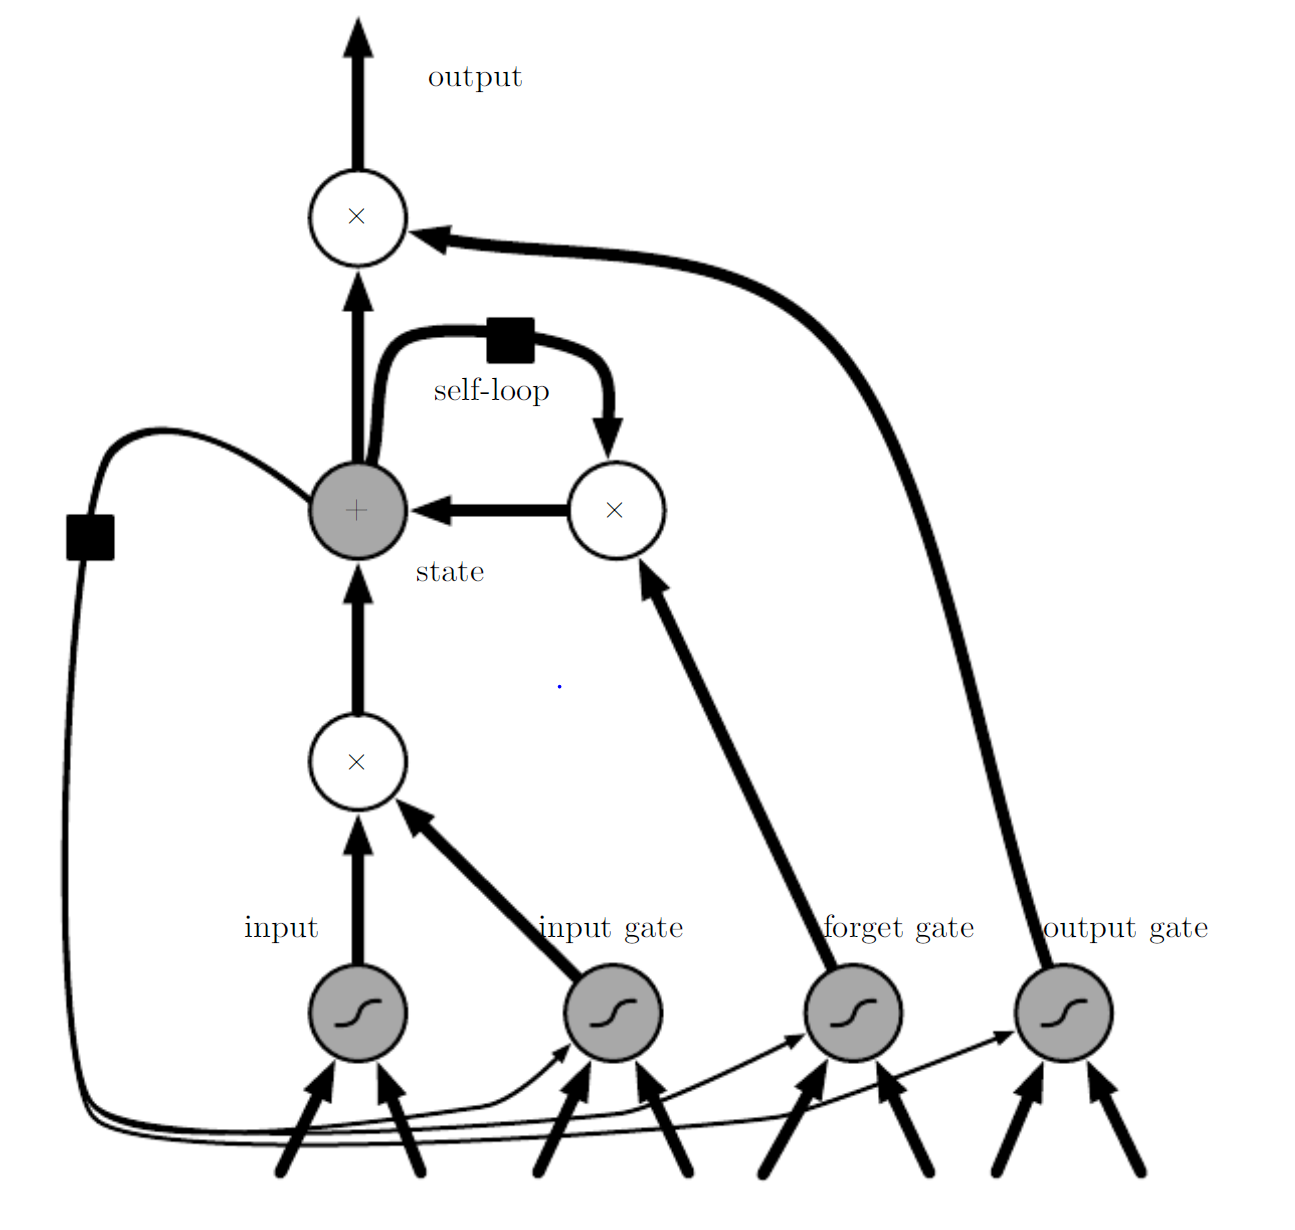
\includegraphics[width = 10 cm]{pic/1.png}
			\caption{Block Diagram of LSTM Cell}
		\end{figure}
		
		LSTM networks have been shown to learn long-term dependencies more easily than the simple recurrent architectures. And we see that in the problem of circular RNA detection, the length of sequence could go fairly long(more than 100000 bases), so we attempt with LSTM rather than other simple gated RNNs.
		
		\section{Our Approach}
		
		We trained a simple LSTM RNN as the classifier, which takes an encoded sequence of DNA as input and produces a single number between 0-1 as prediction.
		
		\subsection{Pipeline}
		
		The network structure is simple: a standard LSTM layer with 64 hidden nodes, stacked with a fully-connected, single-output layer with sigmoid activation. Although being ultimately simple, it is proved to be effective in some other sequence classifying tasks.[4] 
		
		Each DNA base is encoded into a 4-dimensional vector with one-hot encoding. When Alu information is used, an extra dimension is used to indicate whether this base belongs to an Alu sequence.
		
		Of course, samples will be weighted, to balance positive and negative samples. Weights are only determined by numbers of positive and negative sequences, regardless of their length, although it may very greatly.
		
		\subsection{Compromise on limited computation power}
		
		Due to limited computation power, training on the whole dataset, which contains many long sequences with tens or even hundreds of thousands of bases, is beyond our reach. We suggest that only train on short sequences (sequences whose length are under a certain limit) should not worsen the result much, while making training practical.
		
		Although it is obviously a biased sampling of the original dataset, it keeps many features that our network can capture:
		
		\begin{itemize}
			
			\item Statistics about average, such as GC ratio which is proved important[1], is irrelevant to length, thus unaffected.
			
			\item LSTM is theoretically capable for capturing long-range relevance of the sequence, but within a limited training steps it is impossible to "remember" for arbitrarily long. Using sequences longer than LSTM can "remember" cannot make it capture more feature.
			
			\item Slicing from long sequence does keep statistics and short-range relevance, but loses information about absolute position. Using short sequences does not suffer from that.
			
		\end{itemize}
		
		Thus, if we believe that short and long sequences are similar enough, only using short sequences does not differ much from using all sequences, in terms of features that can be captured.
		
		\section{Experiments}
		
		Each model was trained on a single NVIDIA GTX TITAN X, we employed 4 - 8 cards to conduct 10 folds validation test.
		
		\subsection{Effects of setting the longest sequence for training}
		Though LSTM can deal with sequences with changeable length, we still need to set the upbound of RNA sequence we pick due to the video memory of GPU. After observing the sequence distribution of the dataset, we see that the distribution damped heavily at around 100000, so we set the upbound at 100000.
		
		Innitially we tried to train the network with sequences also selected with a length limitation of 100000. It has been shown through experiment that it consumes a great amount of time (2s or so) to train one batch. This made us impossible to train the network economically. Thus, we decided to sample some data from each validation set to train the network, in order to limit the training time in hours. What we've actually done is that we select 1000 blanced sequences from each validation set that we prepared ahead, and we train with sequences sampled from other 9 validation set, and test on the last one with also a balanced ratio. Table 1 has shown the validation result.
		% Table generated by Excel2LaTeX from sheet 'Sheet1'
		\begin{table}[H]
			\centering
			\caption{Trained with a length limitation of 100000}
			\begin{tabular}{l|rrrrrrrrrr|r}
				& \multicolumn{1}{l}{Set 0} & \multicolumn{1}{l}{Set 1} & \multicolumn{1}{l}{Set 2} & \multicolumn{1}{l}{Set 3} & \multicolumn{1}{l}{Set 4} & \multicolumn{1}{l}{Set 5} & \multicolumn{1}{l}{Set 6} & \multicolumn{1}{l}{Set 7} & \multicolumn{1}{l}{Set 8} & \multicolumn{1}{l}{Set 9} & \multicolumn{1}{l}{Mean} \\ \hline \hline
				Accuracy: & 0.7180  & 0.6780  & 0.7780  & 0.8250  & 0.6880  & 0.8280  & 0.7640  & 0.6560  & 0.6890  & 0.6580  & 0.7282  \\
				AUC:  & 0.8385  & 0.7446  & 0.8856  & 0.9177  & 0.7637  & 0.9134  & 0.9369  & 0.7597  & 0.7605  & 0.7550  & 0.8276  \\
				AUPR: & 0.8668  & 0.7045  & 0.9097  & 0.9391  & 0.7436  & 0.9250  & 0.9399  & 0.7719  & 0.7634  & 0.7217  & 0.8286  \\
				F1 score: & 0.7496  & 0.6603  & 0.7874  & 0.8286  & 0.7143  & 0.8277  & 0.8023  & 0.6901  & 0.6631  & 0.7255  & 0.7449  \\
			\end{tabular}%
			\label{tab:addlabel}%
		\end{table}%
		
		\subsection{Effects of using ALU infomation}
		
		We've also attempted to include the information of ALU in this network. The setting we mentioned before consumes more vedio memory, so we have to limit the batch size from 20 to 10. However, we set the number of training samples equally for this experiment and the one listed before for a fair competence. It has been shown from the result below that either this kind of encoding method is not quite reasonable, or due to the increase of encoded vector, this network takes more iters to train.
		
		% Table generated by Excel2LaTeX from sheet 'Sheet1'
		\begin{table}[H]
			\centering
			\caption{Trained with a length limitation of 100000 with ALU info included}
			\begin{tabular}{l|rrrrrrrrrr|r}
				& \multicolumn{1}{l}{Set 0} & \multicolumn{1}{l}{Set 1} & \multicolumn{1}{l}{Set 2} & \multicolumn{1}{l}{Set 3} & \multicolumn{1}{l}{Set 4} & \multicolumn{1}{l}{Set 5} & \multicolumn{1}{l}{Set 6} & \multicolumn{1}{l}{Set 7} & \multicolumn{1}{l}{Set 8} & \multicolumn{1}{l}{Set 9} & \multicolumn{1}{l}{Mean} \\ \hline \hline
				Accuracy: & 0.6809  & 0.6510  & 0.7080  & 0.6780  & 0.7490  & 0.6790  & 0.6510  & 0.6740  & 0.6620  & 0.6760  & 0.6809  \\
				AUC:  & 0.7433  & 0.7395  & 0.7375  & 0.7436  & 0.7287  & 0.7510  & 0.7614  & 0.7156  & 0.7496  & 0.7626  & 0.7433  \\
				AUPR: & 0.3784  & 0.3446  & 0.3727  & 0.3630  & 0.3305  & 0.3913  & 0.4052  & 0.3751  & 0.4035  & 0.4193  & 0.3784  \\
				F1 score: & 0.4405  & 0.3951  & 0.4427  & 0.4371  & 0.4066  & 0.4729  & 0.4416  & 0.4493  & 0.4404  & 0.4791  & 0.4405  \\
			\end{tabular}%
			\label{tab:addlabel}%
		\end{table}%
		
		\subsection{Train with shorter sequences}
		
		We've also tried to limit the length of training sequences to a much more shoter level. This attempt leads to a much more faster training speed and less video memory occupation. One thing worth mention is that due to the unbalanced dataset, negtive cases are usually short, so here the sampling strategy we use varied from 100000 case. This time we used the whole validation set to train, and we upsample positive cases to ensure that there's at least 25\% positve cases in the training batch. It's the same with the validation set, so it becomes unreasonable to compare this result with 100000 cases directly. However, it still looked worse, as the 100000 cases actually haven't reach the stable point yet, but in this case, it's true. We trained with 100 epochs, with 1000 sequences in each epoch.
		
		% Table generated by Excel2LaTeX from sheet 'Sheet1'
		\begin{table}[H]
			\centering
			\caption{Trained with a length limitation of 1500}
			\begin{tabular}{l|rrrrrrrrrr|r}
				& \multicolumn{1}{l}{Set 0} & \multicolumn{1}{l}{Set 1} & \multicolumn{1}{l}{Set 2} & \multicolumn{1}{l}{Set 3} & \multicolumn{1}{l}{Set 4} & \multicolumn{1}{l}{Set 5} & \multicolumn{1}{l}{Set 6} & \multicolumn{1}{l}{Set 7} & \multicolumn{1}{l}{Set 8} & \multicolumn{1}{l}{Set 9} & \multicolumn{1}{l}{Mean} \\ \hline \hline
				Accuracy: & 0.5570  & 0.7880  & 0.7030  & 0.7510  & 0.5420  & 0.6682  & 0.6060  & 0.6510  & 0.6330  & 0.6770  & 0.6576  \\
				AUC:  & 0.7197  & 0.9345  & 0.9261  & 0.8935  & 0.7565  & 0.8461  & 0.7278  & 0.7928  & 0.7365  & 0.7286  & 0.8062  \\
				AUPR: & 0.3612  & 0.8541  & 0.8408  & 0.7796  & 0.3827  & 0.6437  & 0.3125  & 0.4152  & 0.3590  & 0.3601  & 0.5309  \\
				F1 score: & 0.4038  & 0.5638  & 0.5323  & 0.5561  & 0.3893  & 0.4891  & 0.4273  & 0.4655  & 0.4147  & 0.4283  & 0.4670  \\
			\end{tabular}%
			\label{tab:addlabel}%
		\end{table}%
		
		We implemented the ALU test also, unfortunately, no posive effect of ALU have been shown through this result.
		
		% Table generated by Excel2LaTeX from sheet 'Sheet1'
		\begin{table}[H]
			\centering
			\caption{Trained with a length limitation of 1500 with ALU info included}
			\begin{tabular}{l|rrrrrrrrrr|r}
				& \multicolumn{1}{l}{Set 0} & \multicolumn{1}{l}{Set 1} & \multicolumn{1}{l}{Set 2} & \multicolumn{1}{l}{Set 3} & \multicolumn{1}{l}{Set 4} & \multicolumn{1}{l}{Set 5} & \multicolumn{1}{l}{Set 6} & \multicolumn{1}{l}{Set 7} & \multicolumn{1}{l}{Set 8} & \multicolumn{1}{l}{Set 9} & \multicolumn{1}{l}{Mean} \\ \hline \hline
				Accuracy: & 0.5740  & 0.7340  & 0.7000  & 0.6870  & 0.5760  & 0.5960  & 0.6880  & 0.6820  & 0.6600  & 0.8680  & 0.6765  \\
				AUC:  & 0.7055  & 0.9300  & 0.8477  & 0.8462  & 0.7751  & 0.9263  & 0.9234  & 0.9387  & 0.7447  & 0.9308  & 0.8568  \\
				AUPR: & 0.3092  & 0.7970  & 0.6776  & 0.6659  & 0.4080  & 0.8398  & 0.8179  & 0.8615  & 0.3913  & 0.8514  & 0.6620  \\
				F1 score: & 0.4034  & 0.5164  & 0.5033  & 0.4894  & 0.4078  & 0.4834  & 0.5215  & 0.5364  & 0.4276  & 0.7167  & 0.5006  \\
			\end{tabular}%
			\label{tab:addlabel}%
		\end{table}%
		
		% Table generated by Excel2LaTeX from sheet 'Sheet1'
		\begin{table}[H]
			\centering
			\caption{Summary for our experiment}
			\begin{tabular}{l|r|r|r|r}
				& \multicolumn{1}{l}{Table 1} & \multicolumn{1}{l}{Table 2} & \multicolumn{1}{l}{Table 3} & \multicolumn{1}{l}{Table 4} \\ \hline \hline
				Accuracy: & \textbf{0.7282}  & 0.6809  & 0.6576  & 0.6765  \\
				AUC:  & \textbf{0.8276}  & 0.7433  & 0.8062  & 0.8568  \\
				AUPR: & \textbf{0.8286}  & 0.3784  & 0.5309  & 0.6620  \\
				F1 score: & \textbf{0.7449}  & 0.4405  & 0.4670  & 0.5006  \\
			\end{tabular}%
			\label{tab:addlabel}%
		\end{table}%
		
		\section{Discussion}
		
		Our result couldn't be described as satisfactory, but the result is a lot more better than random guessing, which proves that LSTM is indeed learning.
		
		Though we didn't find any previous work using LSTM to predict circRNAs, we know for sure that this is not a rare idea. We don't think our attempts on using LSTM to predict circRNAs have demonstrated that will this approach work well or not. Basiclly due to the limitation of time and GPU resources, it's obvious that we haven't tuned this network quite well. At least the learning curve is still unstable. Some experiments even haven't reach equiblirium.
		
		Another thing worth mentioning is that this dataset is not well designed. Negtive samples are constructed solely by exons, this lead to a situation that negative samples are usually shorter than positive samples. This is not the feature we want to learn here, because this feature will not be helpful when you want to deploy this algorithm to detect circRNA in other situation (You should get longer sequences and it's negtive). One possible approach to deal with this unbalanced distribution is to connect exons close to make longer sequences, it's a shame we didn't have time to try it.
		
		\begin{figure}[H]
			\centering
			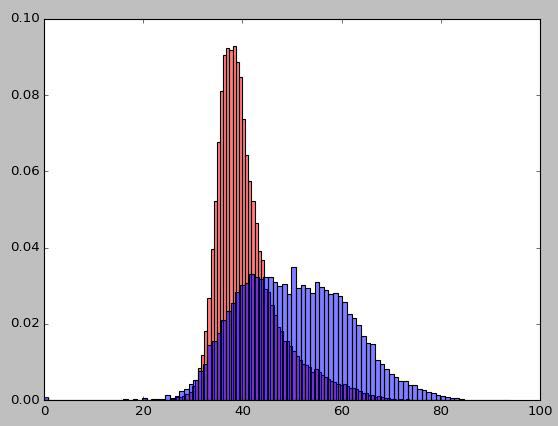
\includegraphics[width = 10cm]{pic/2.jpg}
			\caption{distribution of posive and negtive sequences}
		\end{figure}
		
		One of the most dominant advantages of using LSTM is that we don't design features, it's not a easy work, especially for people who are not familiar with biology. Machines might be able to learn features which maintain a far more general meaning that people could not find, as long as the given data is good. And the disadvantage is that it usually takes great amount of energy and experiments to train a satisfactory network.
		
		\section*{Acknowledgements}
		In this project, Liwei Cai took up the main role for coding. Training and network tuning was conducted by Kaidi Cao. This report was written together. It would be sound that we share a contribution of 50\% each. 
		
		
		\newpage
		
		\section*{Rerferences}
		
		[1] Pan, X., \& Xiong, K. (2015). Predcircrna: computational classification of circular RNA from other long non-coding RNA using hybrid features. Molecular Biosystems, 11(8), 2219-2226.
		
		[2] Liu, Z., Han, J., Lv, H., Liu, J., \& Liu, R. (2016). Computational identification of circular RNAs based on conformational and thermodynamic properties in the flanking introns. Computational Biology \& Chemistry, 61, 221-225.
		
		[3] Ian Goodfellow, Yoshua Bengio, and Aaron Courville . (2016). Deep Learning-2016-Book.
		
		[4] Jason Brownlee. (2016). Sequence Classification with LSTM Recurrent Neural Networks in Python with Keras. Retrieved from http://machinelearningmastery.com/sequence-classification-lstm-recurrent-neural-networks-python-keras/
		
		[5] Team, T. D., Alrfou, R., Alain, G., Almahairi, A., Angermueller, C., \& Bahdanau, D., et al. (2016). Theano: a python framework for fast computation of mathematical expressions.
		
		
	\end{spacing}
\end{document} 